У фермера есть несколько полей, каждое из которых окружено кипарисами.
Также у него есть несколько участков земли, на каждом из которых
растёт ряд кипарисов.
И на полях, и на участках между любыми двумя последовательными кипарисами
растёт ровно одна олива.
Каждый кипарис фермера либо растёт на границе какого-то поля,
либо образуют ряд кипарисов,
а каждая олива находится между какими-то двумя последовательными кипарисами.

Однажды фермер сильно заболел и почувствовал, что он скоро умрёт. За несколько дней до того, 
как он скончался, он позвал своего старшего сына и сказал ему: <<Я оставляю тебе любые $Q$ кипарисов, которые ты выберешь,
и все те оливы, для которых ты выбрал оба соседних с ней кипариса.>> 
На каждом поле и на каждом участке сын может выбрать любой набор кипарисов.
Так как старший сын любит оливы, он хочет выбрать $Q$ кипарисов так,
чтобы унаследовать как можно больше олив.

Напишите программу, которая по данной информации о полях и участках, а также
по количеству кипарисов, которые может выбрать сын, посчитает максимальное
возможное количество олив, которые он может унаследовать.

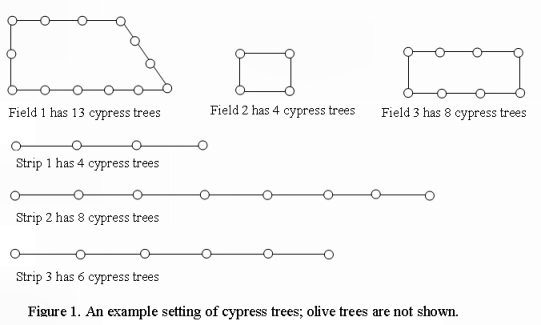
\includegraphics{cypress.jpg}
